\documentclass{article}

\usepackage[utf8]{inputenc}
\usepackage[T1]{fontenc}
\usepackage{amsmath}
\usepackage{amsfonts}
\usepackage{amssymb}
\usepackage[version=4]{mhchem}
\usepackage{stmaryrd}
\usepackage{bbold}
\usepackage{graphicx}
\usepackage{adjustbox}
\usepackage{hyperref}  % For clickable links in TOC
\usepackage{tocloft}   % For TOC formatting
\usepackage{geometry}  % For margins
\usepackage{titlesec}  % For section formatting
\usepackage{fancyhdr}
\usepackage{footmisc}
\usepackage{booktabs}
\usepackage{siunitx}
\usepackage{float}
\usepackage{tikz} 
\usepackage{caption}  
\usetikzlibrary{shapes.geometric, arrows, positioning}  
\DeclareMathOperator*{\argmax}{arg\,max}

\tikzstyle{block} = [rectangle, draw, fill=blue!10,   
     text width=6em, text centered, rounded corners, minimum height=3em]  
\tikzstyle{arrow} = [thick,->,>=stealth]  

% Retrieves visuals 
% visuals

% expected result blue boxes
\usepackage[most]{tcolorbox}
\newtcolorbox{expectedresultsbox}{colback=blue!2!white, colframe=blue!75!black, arc=4mm, boxrule=0.5mm}

% intro black box
\newtcolorbox{solutionoutlinebox}[1][]{%
  enhanced,
  colback=white,
  colframe=black,
  arc=4mm,                % rounded corners
  fonttitle=\bfseries,
  title={\large Solution Outline},
  center title,
  #1
}

% equation system green
\newtcolorbox{systembox}[1][]{%
  enhanced,
  colback=green!2!white,
  colframe=green!75!black,,
  arc=4mm,                % rounded corners
  fonttitle=\bfseries,
  title={ Equilibrium Equations System},
  center title,
  #1
}

% equation system NSS blue
\newtcolorbox{steadystatebox}[1][]{%
  enhanced,
  colback=blue!2!white,
  colframe=blue!75!black,,
  arc=4mm,                % rounded corners
  fonttitle=\bfseries,
  title={Non-Stochastic Steady State System},
  center title,
  #1
}

% equation system LL blue
\newtcolorbox{LLbox}[1][]{%
  enhanced,
  colback=blue!2!white,
  colframe=blue!75!black,,
  arc=4mm,                % rounded corners
  fonttitle=\bfseries,
  title={Log-Linearized System},
  center title,
  #1
}

% equation taylor blue
\newtcolorbox{taylorbox}[1][]{%
  enhanced,
  colback=blue!2!white,
  colframe=blue!75!black,,
  arc=4mm,                % rounded corners
  fonttitle=\bfseries,
  title={Taylor Expansion Theorem},
  center title,
  #1
}

% equation Taylor details (price)
\newtcolorbox{TDbox}[1][]{%
  enhanced,
  colback=blue!2!white,
  colframe=blue!75!black,,
  arc=4mm,                % rounded corners
  fonttitle=\bfseries,
  title={Applying Taylor : Detailed method},
  center title,
  #1
}

% Understanding E_t
\newtcolorbox{Expectationbox}[1][]{%
  enhanced,
  colback=blue!2!white,
  colframe=blue!75!black,,
  arc=4mm,                % rounded corners
  fonttitle=\bfseries,
  title={Law of iterated expectation applied to $E_t$},
  center title,
  #1
}

% Understanding E_t
\newtcolorbox{alternativebox}[1][]{%
  enhanced,
  colback=blue!2!white,
  colframe=blue!75!black,,
  arc=4mm,                % rounded corners
  fonttitle=\bfseries,
  title={The planner problem in conditional form},
  center title,
  #1
}

\newtcolorbox{tobinsbox}[1][]{%
  enhanced,
  colback=blue!2!white,
  colframe=blue!75!black,,
  arc=4mm,                % rounded corners
  fonttitle=\bfseries,
  title={About Tobin's q},
  center title,
  #1
}

\newtcolorbox{responsebox}[1][]{%
  enhanced,
  colback=blue!2!white,
  colframe=blue!75!black,,
  arc=4mm,                % rounded corners
  fonttitle=\bfseries,
  title={Detailed response process},
  center title,
  #1
}

\newtcolorbox{shortbox}[1][]{%
  enhanced,
  colback=white,
  colframe=black,,
  arc=4mm,                % rounded corners
  fonttitle=\bfseries,
  title={In short},
  center title,
  #1
}

\newtcolorbox{interpretationbox}[1][]{%
  enhanced,
 colback=blue!2!white,
  colframe=blue!75!black,,
  arc=4mm,                % rounded corners
  fonttitle=\bfseries,
  title={Economic interpretation : dynamics},
  center title,
  #1
}

\newtcolorbox{RecapBox}[1][]{%
  enhanced,
 colback=blue!2!white,
  colframe=blue!75!black,,
  arc=4mm,                % rounded corners
  fonttitle=\bfseries,
  title={Recap of the system},
  center title,
  #1
}

\newtcolorbox{CondBox}[1][]{%
  enhanced,
 colback=blue!2!white,
  colframe=blue!75!black,,
  arc=4mm,                % rounded corners
  fonttitle=\bfseries,
  title={Recap of the conditions for the ZLB to Bind},
  center title,
  #1
}

\newtcolorbox{takebox}[1][]{%
  enhanced,
 colback=blue!2!white,
  colframe=blue!75!black,,
  arc=4mm,                % rounded corners
  fonttitle=\bfseries,
  title={Main Takeaways},
  center title,
  #1
}

\newtcolorbox{flexbox}[1][]{%
  enhanced,
 colback=green!2!white,
  colframe=green!75!black,,
  arc=4mm,                % rounded corners
  fonttitle=\bfseries,
  title={Impact of price flexiblity on the fiscal multiplier},
  center title,
  #1
}

\newtcolorbox{UCMbox}{colback=white, colframe=black, arc=4mm, boxrule=0.5mm}



% Document styling
\geometry{margin=1in}

% Customize section formatting
\titleformat{\section}
  {\normalfont\Large\bfseries}
  {}
  {0pt}
  {\thesection\quad\rule{\linewidth}{0.4pt}\vspace{0.5em}\newline}
{\normalfont\Large\bfseries}

% adding a header
\pagestyle{fancy}
\fancyhf{}
\lhead{Notes - Macro Models}
\rhead{Romain Fernex}
\cfoot{ \thepage}
\renewcommand{\headrulewidth}{0.8pt}

% Key elements
\title{Macroeconomics - Notes(models)}
\author{Romain Fernex}
\date{February 2025}

\begin{document}

\maketitle
\tableofcontents

\section{RBC model}

\begin{solutionoutlinebox}
\begin{itemize}
    \item \textbf{Households}
    \begin{enumerate}
        \item Solve the utility maximization problem by maximizing with respect to consumption, investments, labor and future capital (bonds might also appear in some settings)
    \end{enumerate}
    \item \textbf{Firms}
    \begin{enumerate}
        \item Solve the profit maximization problem by maximizing with respect to current capital and labor. (The firm is not a monopoly so it does not get to set prices !)
    \end{enumerate}
    \item \textbf{Steady state}
    \begin{enumerate}
        \item Write the equations for the non-stochastic steady state (no time index)
        \item Proceed to log linearize equilibrium equations using non-stochastic steady state equations \footnote{See Isabel and Gustavo's notes for the details}
    \end{enumerate}
\end{itemize}
\end{solutionoutlinebox}

\subsection{Set-up}

\subsubsection{Households}
\begin{itemize}
    \item Goal : Maximize the expected utility of the household over its lifetime by picking a path defining optimal consumption, leisure, investment and capital stock at each period depending on the state of the economy (technology shocks)
    \item Objective function : 
    \begin{equation}
        \max_{C_t,N_t,I_t}E_0[\beta^t(\frac{C_t^{1-\gamma}}{1-\gamma} - \theta\frac{N_t^{1-\psi}}{1+\psi}]
    \end{equation}
    \item Constraints :
    \begin{equation}
    \left\{
    \begin{aligned} 
    \text{Budget : } C_t + I_t = W_tN_t + r_tK_t\\
    \text{Capital Accumulation : } K_{t+1} = (1-\delta)K_t + I_t\\
    \text{Time Endowment : } N_t = 1-L_t
    \end{aligned}
    \right.
    \end{equation} 
\end{itemize}

\subsubsection{Firm}
\begin{itemize}
    \item Goal : Maximize the firm's profit through choosing the optimal combination/level of factor endowments at each period t
    \item Objective function : (no constraints here !)
    \begin{equation}
        \max_{K_t, N_t}\pi_t = Y_t - \tilde{R}_tK_t - W_tN_t
    \end{equation}
\end{itemize}

\subsubsection{Steady state}
\begin{systembox}
    \begin{itemize}
        \item \textbf{Euler Equation :} $C_t^{-\gamma} = E_t[\beta C_{t+1}^{-\gamma}(r_{t+1}+1-\delta)]$
        \item \textbf{Work/Leisure tradeoff :} $\theta N_t^{-\psi} = W_tC_t^{-\gamma}$
        \item \textbf{Time endowment constraint :} $L_t = 1-N_t$
        \item \textbf{Flow budget constraint :} $C_t+I_t = Y_t$ [obtained from the firm's profit equation given that profit is null, combined with BC in equation (2)]
        \item \textbf{Capital accumulation constraint :} $K_{t+1} = I_t + (1-\delta)K_t$
        \item \textbf{Firm's MPK :} $\alpha\frac{Y_t}{K_t} = r_t$
        \item \textbf{Firm's MPN :} $(1-\alpha)\frac{Y_t}{N_t} = W_t$ 
        \item \textbf{Production function :} $Y_t = Z_tK_t^{\alpha}N_t^{1-\alpha}$
        \item \textbf{Law of motion of productivity/technology :} $ln(Z_t) = \rho ln(Z_{t-1})+\epsilon_t$
    \end{itemize}
\end{systembox}
\textbf{Non-stochastic steady state}
\begin{itemize}
    \item Goal : We wish to find the point around wish the economy fluctuates to see how shocks create deviations from this equilibrium (how fast does the economy converge back to its steady state etc..)
    \item Method : see "Tricks \& Results" part
\end{itemize}

\textbf{Log-linearization}
\begin{itemize}
    \item Goal : Transform our system of non-linear equations in a system of linear ones. This helps greatly for our analysis (for instance it helps with moment calculation as we have a linear expectation term)
    \item Limitations : Log linearization is only valid if 
    \begin{enumerate}
        \item We only have small deviations from steady state
        \item The model does not have significant nonlinearities
    \end{enumerate}
    \item Method : See "Tricks \& Results" part \footnote{For additional details, please refer to Gustavo and Isabel's notes}
\end{itemize}

\subsection{Tricks and results}

\subsubsection{Households}
\begin{enumerate}
    \item Simplify the constraint : Take the capital accumulation constraint and express $I_t$ as a function of the other variables. Then substitute $I_t$ in the budget constraint to get rid of investments. 
    \begin{expectedresultsbox}
    \begin{equation}
        \textcolor{blue}{\textbf{New constraint : }} W_tN_t + r_tK_t + (1-\delta)K_t = C_t + K_{t+1}
    \end{equation}
    \end{expectedresultsbox}
    \item Derive the FOC with respect to $C_t$ to obtain the shadow value $\lambda_t$ of increasing consumption.
    \begin{expectedresultsbox}
    \begin{equation}
        \textcolor{blue}{\textbf{Expected result : }} C_t^{-\gamma} = \lambda_t
    \end{equation}
    \end{expectedresultsbox}
    \item Derive the FOC with respect to $K_t$ to get the Euler Equation. Replace $\lambda_{t}$ and $\lambda{_{t+1}}$ using (1)
    \begin{expectedresultsbox}
    \begin{equation}
        \textcolor{blue}{\textbf{Expected result : }} \underbrace{C_t^{-\gamma}}_{=\lambda_t} = E_t[\beta \underbrace{C_{t+1}^{-\gamma}}_{=\lambda_{t+1}}(r_{t+1}+1-\delta)]
    \end{equation}
    \end{expectedresultsbox}
    \item Derive the FOC with respect to $N_t$ to get the leisure/work tradeoff equation.
    \begin{expectedresultsbox}
    \begin{equation}
        \textcolor{blue}{\textbf{Expected result : }} \theta N_t^{-\psi} = W_tC_t^{-\gamma}
    \end{equation}
    \end{expectedresultsbox}
\end{enumerate}

\subsubsection{Firm}
\begin{enumerate}
    \item Derive the FOC with respect to $K_t$ to find the marginal product of capital (MPK)
    \begin{expectedresultsbox}
    \begin{equation}
        \textcolor{blue}{\textbf{Expected result : }} \alpha\frac{Y_t}{K_t} = \tilde{R}_t \,\footnotemark
    \end{equation}
    \end{expectedresultsbox}
    \item Derive the FOC with respect to $N_t$ to find the marginal product of labor (MPN) 
    \begin{expectedresultsbox}
    \begin{equation}
        \textcolor{blue}{\textbf{Expected result : }} (1-\alpha)\frac{Y_t}{N_t} = W_t 
    \end{equation}
    \end{expectedresultsbox}   
\end{enumerate}

\footnotetext{$\alpha$ corresponds to the share of production due to capital (generally fixed to 2/3)}


\subsubsection{Steady state}

\textbf{Non-stochastic steady state}
\begin{enumerate}
    \item To obtain the system of non-stochastic steady state equation you need to remove all time/period indexes from the variables and rearrange each equation when needed
    \item For the law of motion of productivity : The $\epsilon$ term disappears as there are no shocks in steady state 
    \begin{itemize}
        \item BEWARE : (assuming $\rho \neq 1$) you can't divide by $log(Z)$ as we can't tell whether it is equal to 0. Therefore move log on the same side and divide by the constant to end up with $Z=1$
    \end{itemize}
\end{enumerate}
\begin{steadystatebox}
 \begin{itemize}
        \item \textbf{Euler Equation :} $1 = \beta(r+1-\delta) = \beta R$
        \item \textbf{Work/Leisure tradeoff :} $\theta N^{-\psi} = WC^{-\gamma}$
        \item \textbf{Time endowment constraint :} $L=1-N$
        \item \textbf{Flow budget constraint :} $C+I = Y$ 
        \item \textbf{Capital accumulation constraint :} $I = \delta K$
        \item \textbf{Firm's MPK :} $\alpha\frac{Y}{K} = r$
        \item \textbf{Firm's MPN :} $(1-\alpha)\frac{Y}{N} = W$ 
        \item \textbf{Production function :} $ZK^{\alpha}N^{1-\alpha}$
        \item \textbf{Law of motion of productivity/technology :} $Z=1$
    \end{itemize}
\end{steadystatebox}
\textbf{Log-Linearization}
    \begin{enumerate}
        \item We replace the variables by their exponential forms ($X_t = Xe^{\hat{X}_t}$)
        \item We cancel out constant terms using steady state equations
        \item If we have multiplications of variables by one another we use Taylor 
        \begin{taylorbox}
            \textbf{Taylor's Theorem:} For \(f \in C^{n+1}(I)\) where \(I\) is an open interval containing \(a\):
            \[f(x) = \sum_{k=0}^{n} \frac{f^{(k)}(a)}{k!}(x-a)^k + \frac{f^{(n+1)}(\xi)}{(n+1)!}(x-a)^{n+1}\text{ where \(\xi\) lies between \(a\) and \(x\).}\]
            \textbf{Conditions:}
            \begin{itemize}
            \item \(f^{(n+1)}\) exists on \(I\)
            \item \(f\) is continuous on \([a,x]\)
            \end{itemize}
        \end{taylorbox}
        \item Otherwise, using the log is sufficient to find back what we need
        \item Note : for the log linearization of the EE, it is useful to use the following expression which is also obtained through log-linearization $R\hat{R}_{t+1} = r\hat{r}_{t+1}$ \footnote{See Gustavo's note, p.10}
\end{enumerate}
\begin{LLbox}
    \begin{itemize}
        \item \textbf{Euler Equation :} $\hat{C}_t=E_t[\hat{C}_{t+1}-\frac{1}{\gamma}\hat{R}_{t+1}] $
        \item \textbf{Work/Leisure tradeoff :} $\psi \hat{N}_t = \hat{W}_t-\gamma\hat{C}_t$
        \item \textbf{Time endowment constraint :} $\hat{N}_t=-\frac{L}{N}\hat{L}_t$
        \item \textbf{Flow budget constraint :} $\frac{C}{Y}\hat{C}_t+\frac{I}{Y}\hat{I}_t=\hat{Y}_t$ 
        \item \textbf{Capital accumulation constraint :} $\hat{K}_{t+1}=(1-\delta)\hat{K}_t+\delta\hat{I}_t$
        \item \textbf{Interest rate (firm's MPK):} $\hat{r}_t=\hat{Y}_t-\hat{K}_t$
        \item \textbf{wage (Firm's MPN) :} $\hat{W}_t=\hat{Y}_t-\hat{N}_t$ 
        \item \textbf{Production function :} $\hat{Y}_t=\hat{Z}_t+\alpha\hat{K}_t+(1-\alpha)\hat{N}_t$
        \item \textbf{Law of motion of productivity/technology :} $\hat{Z}_t=\rho\hat{Z}_{t-1}+\epsilon_t$ \footnotemark
        \item \textbf{Gross interest rate} $\hat{R}_t=\frac{r}{R}\hat{r}_t$
    \end{itemize}
\end{LLbox}

\footnotetext{be careful, we keep $\epsilon$ as is here, we do not log-linearize it}

%------------------------------------------------------------------


\section{New-Keynesian model}

\begin{solutionoutlinebox}
\begin{itemize}
    \item \textbf{Households}
    \begin{enumerate}
        \item Intratemporal  : Solve the expenditure minimization problem for Household by minimizing with respect to consumption of a given good at a given period ($C_s(i)$)
        \item Intertemporal : Solve the utility maximization problem by maximizing expected utility with respect to aggregate consumption, labor and bonds 
    \end{enumerate}
    \item \textbf{Firms}
    \begin{enumerate}
        \item Flexible prices : Solve the profit maximization problem, assuming that prices can be adjusted at each period, by maximizing with respect to the price of a given good at a given period ($P_t(i)$)
        \item Sticky prices : Solve the profit maximization problem, assuming prices have a non null probability of carrying over to the next period, by maximizing with respect to the price of a given good at the period the price is set - right before the carryover($P_t(i)$)
    \end{enumerate}
    \item \textbf{Steady State}
    \begin{enumerate}
        \item Log Linearization : same process as with RBC with a little twist for adjusted prices\footnote{See "Results \& Methods" part for the details}
        \item Phillips curve : find the equation from the phillips curve based based on the log-linearized system. It shows how current inflation depends on expected future inflation and current economic conditions (marginal cost)
    \end{enumerate}
\end{itemize}
\end{solutionoutlinebox}

\subsection{Set-up}

\subsubsection{Households}

\textbf{A) The Expenditure Minimization Problem}

\begin{itemize}
    \item Goal : Minimize total expenditures across all goods while achieving a certain level of aggregate consumption
    \item Objective function : 
    \begin{equation}
        \min_{C_s(j)}\int_0^1P_s(i)C_s(i)di 
    \end{equation}
    \item Constraint : 
    \begin{equation}
        C_s = (\int_0^1C_s(i)^{\frac{\theta-1}{\theta}})^{\frac{\theta}{\theta-1}} \text{ with $C_s$ the desired aggregate consumption level}\,\footnotemark
    \end{equation}
\end{itemize}

\textbf{B) The Utility Maximization Problem}

\begin{itemize}
    \item Goal : maximize expected utility over the lifetime of the consumer
    \item objective function : 
    \begin{equation}
        \max_{N_s,C_s,B_s}E_t[\sum_{s=t}^\infty\beta^{s-t}(\frac{C_s^{1-\gamma}-1}{1-\gamma}-\phi\frac{N_s^{1+\psi}}{1+\psi})]\,\footnotemark
    \end{equation}
    \item Constraints : 
    \begin{equation}
    \left\{
    \begin{aligned}
        &\text{Budget : } R_{s-1}B_{s-1}+W_sN_s+D_s = T_s + B_s +P_sC_s \text{ with $T_s$ = taxes}\\
        &\text{Initial condition : } B_{t-1} = 0\\
        &\text{TVC : } \lim_{s\to\infty} B_s(\Pi_{i=0}^s R_{s-i}) = 0
    \end{aligned}
    \right.
    \end{equation}
\end{itemize}

\footnotetext{$\theta$ is the elasticity of substitution across goods (the lower it is, the more market power firms will have}
\footnotetext{$\gamma$ is the inverse of IES (intertemporal elasticity of substitution), $\psi$ the inverse of the Frisch elasticity of labor supply(the lower it is, the less responsive the household is to wage changes) and $\phi$ governs the degree of wage rigidity}

\subsubsection{Firms}

\textbf{A) The Profit Maximization Problem : Flexible Prices}

\begin{itemize}
    \item Goal : set optimal prices at each period so as to maximize the companies profit (monopoly behavior : does not take prices as given)
    \item Objective function : 
    \begin{equation}
        \max_{P_s(i),N_s(i)} \pi_s(i) = (1+\tau)P_s(i)Y_s(i) - W_sN_s(i) 
    \end{equation}
    \item Constraints : 
    \begin{equation}
    \left\{
    \begin{aligned}
        &\text{Production function : }Y_s(i) = A_sN_s(i) \,\footnotemark \\
        &\text{Technology flow : }ln (A_s) = \rho_Aln(A_{s-1}) + \epsilon_s^a \,\footnotemark \\
        &\text{Monopoly : }Y_s(i) = C_s(i) = (\frac{P_s}{P_s(i)})^{\theta}C_s \,\footnotemark
    \end{aligned}
    \right.
    \end{equation}
\end{itemize}

\footnotetext{$A_s$ is productivity/technology at period s}
\footnotetext{$\epsilon$ represents technology shocks, $\rho$ represents determines how much of the previous period's technology level carries over to the current period (if 0 shocks are short-lived}
\footnotetext{The firm behaves monopolistically so it equates quantities produced with quantities demanded}

\textbf{B) The Profit Maximization Problem : Sticky Prices}
\begin{itemize}
    \item Goal : find the optimal price that maximizes profits over time given the fact that price can't be adjusted for a certain number of periods
    \item Problem : 
    \begin{equation}
        X_t(i) = \argmax_{P_t(i)} E_t[\sum_{s=t}^\infty (\lambda\beta)^{s-t}\frac{C_s^{-\gamma}/P_s}{C_t^{-\gamma}/P_t}((1+\tau)P_t(i) - \frac{W_s}{A_s})(\frac{P_t(i)}{P_s})^{-\theta}C_s] \,\footnotemark\,\footnotemark
    \end{equation}
\end{itemize}

\footnotetext{alternative notation : $\Lambda_{s} = \beta^{s-t}(\frac{C_{s}^{-\gamma}/P_{s}}{C_t^{-\gamma}/P_t})$ and $\forall s, \tilde{c_{s}}(i) = (\frac{P_t(i)}{P_s})^{-\theta}C_s $}
\footnotetext{$\Lambda_{s}$ is named the relevant stochastic discount factor for nominal payoff, $\tilde{c_{s}}(i)$ is the demand for good i conditional on the price of this good not varying over time}

\subsubsection{Planner}
\begin{itemize}
    \item objective : allocate consumption to the representative household and labor to the firms in a way that maximizes the well-being of the household. The allocation it chooses is the efficient allocation and can be compared to the allocation obtained in the decentralized case to identify inefficiencies. 
    \item objective function : 
    \begin{equation}
        \max_{C_t,N_t} U(C_t,N_t)
    \end{equation}
    \item constraints : 
    \begin{equation}
    \left\{
    \begin{aligned}
        \textbf{Aggregate Consumption Constraint : }C_t &= \left(\int_0^1C_t(i)^{\frac{\theta-1}{\theta}}di \right)^{\frac{\theta}{\theta-1}}\\
        \textbf{Production Function for each good i : }C_t(i) &= A_tN_t(i), \forall i\in[0,1]\\
        \textbf{Aggregate Labor Constraint : } N_t&=\int_0^1N_t(i)di
    \end{aligned}  
    \right.
    \end{equation}
    \item results : at optimality households consume the same quantity of all goods, allocate the same amount of labor to all firms (why ? : 1) goods enter utility function in the same way, 2)concave utility) and the marginal disutility of labor equals its marginal benefit. 
    \item potential inefficiencies in decentralized equilibrium : 
    \begin{enumerate}
        \item Price stickiness 
        \item Market power (monopolies)
        \item Price dispersion (linked to price stickiness but may be problematic even in the period t-1)
    \end{enumerate}
\end{itemize}

\subsubsection{Steady state}
\begin{systembox}
    \begin{itemize}
        \item Demand for a differentiated good : $C_s(i) = (\frac{P_s}{P_s(i)})^{\theta}C_s$
        \item Euler Equation (inter-temporal) : $E_t\left[\beta\frac{R_s}{\Pi_{s+1}}C_{s+1}^{-\gamma}\right] = C_s^{-\gamma}$
        \item Labor supply : $\phi N_s^{\psi}  = \frac{C_s^{-\gamma}}{P_s}W_s$
        \item Labor demand (per firm) : $N_t(i) = \frac{1}{A_t}(\frac{P_t(i)}{P_t})^{-\theta}C_t$
        \item Labor market clearing : $N_t = \int_0^1N_t(i)di$
        \item Price index : $P_t = (\int_0^1P_t(i)^{1-\theta}di)^{\frac{1}{1-\theta}}$
        \item Adjusted price (sticky) : $X_t(i) = \frac{\theta}{(\theta-1)(1+\tau)}\frac{E_t[\sum_{s=t}^\infty(\lambda\beta)^{s-t}\frac{W_s}{A_s}P_s^{\theta}C_s^{1-\gamma}]}{E_t[\sum_{s=t}^{\infty}(\lambda\beta)^{s-t}P_s^{\theta-1}C_s^{1-\gamma}]}$
        \item Flexible price : $P_t(i) = \frac{1}{1+\tau}\frac{\theta}{\theta-1}\frac{W_t}{A_t}$
        \item Taylor rule (Monetary policy) : $R_t=R\Pi_t^{\phi_\pi}e^{\epsilon_t^r}$
    \end{itemize}
\end{systembox}
\textbf{Non-stochastic steady state and Log-linearization}
\begin{itemize}
    \item Goal : same as with the RBC model
    \item Method : see "Tricks \& Results" part
\end{itemize}
\textbf{Phillips curve}
\begin{itemize}
    \item Goal : show current inflation depends on expected future inflation and current economic conditions (marginal cost)
    \item Method (how to get it) : see "Tricks \& Results" part
\end{itemize}



\subsection{Tricks and results}

\subsubsection{Households}

\textbf{A) The Expenditure Minimization Problem}
\begin{enumerate}
    \item Derive the FOC wrt. $C_s(i)$ : be mindful that we are considering a single good in a single period so the integral in the left hand term can be safely ignored (it's as if we were to take a specific term in a sum
    \begin{expectedresultsbox}
    \begin{equation}
        \textcolor{blue}{\textbf{Expected result : }} C_s(i) = (\frac{\lambda_s}{P_s(i)})^{\theta}C_s
    \end{equation}
    \end{expectedresultsbox}
    \item Substitute the result obtained for $C_s(i)$ in the constraint to find an expression for $\lambda_s$
    \begin{expectedresultsbox}
    \begin{equation}
        \textcolor{blue}{\textbf{Expected result : }} \lambda_s = P_s \,\footnotemark
    \end{equation}
    \end{expectedresultsbox}
    \item Substitute $\lambda_s$  in the expression for the optimal $C_s(i)$ that we found earlier
    \item Substitute this new expression for $C_s(i)$ in the objective function
    \begin{expectedresultsbox}
    \begin{equation}
        \textcolor{blue}{\textbf{Expected result : }} TE = P_sC_s
    \end{equation}        
    \end{expectedresultsbox}
\end{enumerate}

\footnotetext{interpretation : the shadow value of increasing aggregate consumption is equal to the price index}

\textbf{B) The Utility Maximization Problem}
\begin{enumerate}
    \item FOC wrt $C_s$ : define $\lambda_s$ as a function of the rest
    \begin{expectedresultsbox}
    \begin{equation}
        \textcolor{blue}{\textbf{Expected result : }} \lambda_s = \frac{C_s^{-\gamma}}{P_s}
    \end{equation}
    \end{expectedresultsbox}
    \item FOC wrt $N_s$ (work/leisure tradeoff): equalize marginal cost (hours spent working) with marginal benefit of labor (consumption derived from labor income) $\xrightarrow{}$ can't improve situation by working more/less
    \begin{expectedresultsbox}
    \begin{equation}
        \textcolor{blue}{\textbf{Expected result : }} \phi N_s^{\psi}  = \frac{C_s^{-\gamma}}{P_s}W_s
    \end{equation}
    \end{expectedresultsbox}
    \item FOC wrt $B_s$ (Euler equation) : use (8) and equalize marginal expected utility of future consumption and marginal benefit of current consumption $\xrightarrow{}$ can't improve situation by consuming more now or in the future
    \begin{expectedresultsbox}
    \begin{equation}
        \textcolor{blue}{\textbf{Expected result : }} E_t\left[\beta\frac{R_s}{\Pi_{s+1}}C_{s+1}^{-\gamma}\right] = C_s^{-\gamma}\,\footnotemark
    \end{equation}
    \end{expectedresultsbox}
\end{enumerate}

\footnotetext{$\Pi_{s+1} = \frac{P_{s+1}}{P_s}$ and corresponds to inflation}

\subsubsection{Firms}

\textbf{A) The Profit Maximization Problem : Flexible Prices}
\begin{enumerate}
    \item Rearrange the problem to get rid of $N_s(i)$ and the constraint : to do that replace $C_s(i)$ by its constraint value and use the production function to express $N_s(i)$ as a function of other variables 
    \begin{expectedresultsbox}
    \begin{equation}
        \textcolor{blue}{\textbf{Expected result : }} \max_{P_s(i)} [(P_s(i)(1+\tau) - \frac{W_s}{A_s}]P_s(i)^{-\theta}P_s^{\theta}C_s
    \end{equation}
    \end{expectedresultsbox}
    \item Find the FOC wrt to $P_s(i)$ : consumption and price aggregates cancel out, then just rearrange the terms
    \begin{expectedresultsbox}
    \begin{equation}
        \textcolor{blue}{\textbf{Expected result : }} P_s(i) = \frac{1}{1+\tau}\frac{\theta}{\theta-1}\frac{W_s}{A_s}
    \end{equation}
    \end{expectedresultsbox}
\end{enumerate}

\textbf{B) The Profit Maximization Problem : Sticky Prices}
\begin{itemize}
    \item Deriving the FOC with respect to $P_t(i)$ : 
    \begin{enumerate}
        \item Start by canceling out aggregate terms with index t 
        \item divide by $P_t(i)^{-\theta-1}$ on each side
        \item Move all terms that do not depend on s outside of the expectation 
        \item Put the remaining $P_t(i)$ on one side and rearrange term to express it as a function of all other remaining terms
    \end{enumerate}
    \begin{expectedresultsbox}
    \begin{equation}
        \textcolor{blue}{\textbf{Expected result : }} X_t(i) = \frac{\theta}{(\theta-1)(1+\tau)}\frac{E_t[\sum_{s=t}^\infty(\lambda\beta)^{s-t}\frac{W_s}{A_s}P_s^{\theta}C_s^{1-\gamma}]}{E_t[\sum_{s=t}^{\infty}(\lambda\beta)^{s-t}P_s^{\theta-1}C_s^{1-\gamma}]}
    \end{equation}
    \end{expectedresultsbox}
\end{itemize}

\subsubsection{Planner}
\begin{enumerate}
    \item Solving the planners problem : set up the lagrangian with a costate variable for each of the three constraints. Be careful for the production constraint as you need to introduce a constraint for each good.
    \begin{expectedresultsbox}
        \textcolor{blue}{\textbf{expected result : }}  $\begin{aligned}\mathcal{L} &= U(C_t, N_t) + \lambda_t \left[ C_t - \left(\int_0^1 C_t(i)^{\frac{\theta-1}{\theta}}\, di \right)^{\frac{\theta}{\theta-1}} \right] \ \\[1em]&\quad+ \int_0^1 \mu_t(i) \left[ C_t(i) - A_t\, N_t(i) \right]\, di  + \nu_t \left[ N_t - \int_0^1 N_t(i)\, di \right]\end{aligned}$ 
    \end{expectedresultsbox}
    \item Take the FOC's with respect to $C_t, N_t, N_t(i)$ and use costates to find back the following optimality conditions : 
    \begin{expectedresultsbox}
         \textcolor{blue}{\textbf{expected result : }} \begin{equation}
        \left\{
        \begin{aligned}
            C_t(i)&=C_t, \forall i\in[0,1]\\
            N_t(i) &= N_t\\
            -U_{n,t}&=A_tU_{c,t}
        \end{aligned}   
        \right.
        \end{equation}
    \end{expectedresultsbox}
\end{enumerate}

\subsubsection{Steady state}
\textbf{A) Non-stochastic steady state}
\begin{enumerate}
    \item We start by proceeding in the same way as in the RBC model (remove time indexes)
    \item For adjusted prices : move the constant terms (W, A, P, and C) outside of the sum. The sums can then be canceled out, along with the term in P and C. 
    \item For aggregate labor and prices : Notice that $P_s(i), X_s(i)$ and $N_s(i)$ do not depend on i (see equation 24,25). In other words, at equilibrium, all firms will price in the same way and demand the same quantity of labor. This entails that : $\forall i, N(i) = N$ and $P(i)=P$ in the non-stochastic steady state.
\end{enumerate}
\begin{steadystatebox}
    \begin{itemize}
        \item Demand for a differentiated good : $C(i) = (\frac{P(i)}{P})^{-\theta}C$
        \item Euler Equation (inter-temporal) : $\beta \frac{R}{\Pi}=1$
        \item Labor supply : $\phi N^{\psi} = \frac{C^{-\gamma}}{P}W$
        \item Labor demand (per firm) : $N(i) = \frac{C}{A} = \frac{Y}{A}$
        \item Labor market clearing : $N=\int_0^1N(i)di$
        \item Price index : $P = (\int_0^1P(i)^{1-\theta}di)^{\frac{1}{1-\theta}}$
        \item Adjusted price (sticky) : $X = X(i) = \frac{\theta}{(\theta-1)(1+\tau)}\frac{W}{A}$
        \item Flexible price : same as adjusted price ! $X=P=P(i)$
        \item Taylor rule (monetary policy) : $1=\Pi$ \footnote{The gross inflation rate $\Pi$ is equal to 1 so there is zero net inflation}
    \end{itemize}
\end{steadystatebox}
\textbf{B) Log-linearization}
\begin{enumerate}
    \item The overall method is the same as before, however some additional tricks are necessary (especially for prices).
    \item Euler Equation : 
    \begin{itemize}
        \item Replace variables by their exponential form $(Xe^{x_t})$ and cancel out constant terms using steady state equations
        \item For efficacy, it is preferable to group together exponents and THEN use Taylor
        \begin{expectedresultsbox}
     \textcolor{blue}{\textbf{Trick n°1 : }}Take $e^{r_t-\pi_t-\gamma c_t}$ which gives $(r_t-\pi_t)-\gamma c_t + 1$ (using Taylor)\footnote{WARNING : here $r_t$ is just the equivalent of $\hat{R}_t$ which is the notation we used for the RBC model}
        \end{expectedresultsbox}
    \end{itemize}
    \item Adjusted price : 
    \begin{itemize}
        \item The first steps are the same as the Euler equation (substitute variables in exp form, cancel out constants, group exponentials in each sum and use Taylor)
        \item We rearrange the sums and use Taylor a second time but for functions of the form$\frac{1}{1+x}$ (see details below)
        \begin{TDbox}
            We start by noting : 
            \begin{equation}
                \Phi_s \equiv (1-\gamma)c_s + (\theta-1)p_s
            \end{equation}
            This gives us the following equation : 
            \begin{equation}
                1+x_t(i)=\frac{ \sum_{s=t}^\infty (\lambda\beta)^{s-t}(1+\Phi_s+w_s-a_s)}{\lambda\beta)^{s-t}(1+\Phi_s)}
            \end{equation}
            For improved clarity, we now set the following : 
            \begin{equation}
            \left\{
            \begin{aligned}
               S \equiv \sum_{s=t}^\infty (\lambda\beta)^{s-t} \\
               \epsilon_N \equiv \sum_{s=t}^\infty (\lambda\beta)^{s-t} (\Phi_s+w_s-a_s)\\
               \epsilon_D \equiv \sum_{s=t}^\infty (\lambda\beta)^{s-t} \Phi_s
            \end{aligned}
            \right.
            \end{equation}
            This gives us this, which we will simplify using Taylor : 
            \begin{equation}
                1+x_t(i) = \frac{S +               \epsilon_N}{S +               \epsilon_D}
            \end{equation}
            We can rewrite this to take the following form : 
            \begin{equation}
                1+x_t(i) = \frac{S(1+\epsilon_N/S)}{S(1+\epsilon_D/S)} = \frac{(1+\epsilon_N/S)}{(1+\epsilon_D/S)}
            \end{equation}
            Now we can linearize the denominator using Taylor \footnote{Please refer to the math appendix 4.1} on $\frac{1}{1+\epsilon_D/S}$ (we take $X\equiv \epsilon_D/S$) 
            \begin{equation}
                \frac{1}{1+\epsilon_D/S}\sim (1-\epsilon_D/S)
            \end{equation}
            Now, we multiply it with the numerator and get rid of higher order terms :
            \begin{equation}
            \frac{(1+\epsilon_N/S)}{(1+\epsilon_D/S)} = (1-\epsilon_D/S)(1+\epsilon_N/S) = 1+\frac{\epsilon_N}{S}-\frac{\epsilon_D}{S} = 1 + \frac{\epsilon_N-\epsilon_D}{S}
            \end{equation}
            Notice the following : 
            \begin{equation}
                \epsilon_N-\epsilon_D = \sum_{s=t}^\infty (\lambda\beta)^{s-t}(w_t-a_t)
            \end{equation}
        \end{TDbox}
        \item Following the second Taylor expansion we have this expression : 
        \begin{expectedresultsbox}
        \begin{equation}
            \textcolor{blue}{\textbf{Expected result: }} 1 + x_t(i) = 1 + \frac{\sum_{s=t}^\infty (\lambda\beta)^{s-t}(w_t-a_t)}{\sum_{s=t}^\infty (\lambda\beta)^{s-t}}
        \end{equation}
        \end{expectedresultsbox}
        \item We are now left with two little steps : cancel out the ones and rewrite the denominator. For the latter, notice that it is a geometric series and can be rewritten as $\frac{1}{1-\lambda\beta}$\footnote{See math appendix 4.2}
        \item Just flip the denominator and you're done ! 
    \end{itemize}
    \item Price index : 
        \begin{itemize}
            \item Right-most equality : Write variables in exponent form and get rid of constant terms based on non-stochastic steady state. Then, use the first order Taylor approximation and cancel out the ones.
            \item Left-most equality, we use the fact that, at equilibrium :
            \begin{equation}
                P_t^{1-\theta} = ((1-\lambda)X_t^{1-\theta} + \lambda P_{t-1}^{1-\theta}) \,\footnotemark
            \end{equation}
            \item So at the NS steady state we get : $P^{1-\theta} = (1-\lambda)X^{1-\theta} + \lambda P^{1-\theta}$. From there we just apply the usual method (exp + NS steady state cancellation + Taylor expansion)
        \end{itemize}
    \item Expected end result : 
\end{enumerate}
\begin{LLbox}
    \begin{itemize}
        \item Demand for a differentiated good : $c_t(i) = -\theta(p_t(i)-p_t)+c_t$
        \item Euler equation : $c_t = E_t[-\frac{1}{\gamma}(r_t-\pi_{t+1})+c_{t+1}]$
        \item Labour supply : $w_t-p_t = \psi n_t + \gamma c_t$
        \item Labour market clearing : $n_t = \int_0^1n_t(i)di$ 
        \item Labour demand : $n_t(i)=c_t-a_t-\theta(p_t(i)-p_t)$
        \item Price index : $p_t = \int_0^1p_t(i)di = \lambda p_{t-1} + (1-\lambda)x_t$
        \item Adjusted price (sticky)\footnote{notice that neither adjusted prices nor flexible ones depend on the firm, all price the same way !} : $x_t(i) = (1-\lambda\beta)E_t[\sum_{s=t}^\infty(\lambda\beta)^{s-t}(w_s-a_s)]$ and $x_t = x_t(i)$
        \item Flexible price : $p_t^f=p^f_t(i)=w_t^f-a_t$
        \item Taylor rule (monetary policy) : $r_t = \phi_{\pi}\pi_t+\epsilon_t^{r}$
    \end{itemize}
\end{LLbox}

\footnotetext{For additional details on how we get this expression, look at slide 19 in the lecture notes}

\textbf{C) Phillips curve (normal version)}
\begin{enumerate}
    \item Start from $x_t$ after log linearization
    \item Split the sum with the term where s=t on one side, and all the others on the other side
    \item Move one of the $\lambda\beta$ outside the sum and outside the expectation
    \item Managing expectations : 
    \begin{itemize}
        \item For the term where s=t you can remove the expectation (it does not depend on future periods)
        \item For the other term : we  use the law of iterated expectation to make $E_{t+1}$ appear in our expression so we'll be able to substitute it with $x_{t+1}$ in the next step.
        \begin{Expectationbox}
            Remember that $E_t$ is a conditional expectation that can also be noted in the following way :
            \begin{equation}
                E_t \equiv E[.|z_t] \text{ with $z_t$ the history of $Z$ until period t included} \,\footnote{for more details, see Pset 1, Problem 3}
            \end{equation}
            Thus, it becomes possible to use the law of iterated expectation in the following way
            \begin{equation}
                E_t =E[E(.|z_{t+1})|z_t] =  E_t[E_{t+1}] 
            \end{equation}
        \end{Expectationbox}
    \end{itemize}
    \item Move one $\lambda\beta$ coefficient outside of $E_t[E_{t+1}]$ and notice that we get exactly $\lambda\beta E_t[x_{t+1}]$ 
    \begin{expectedresultsbox}
    \begin{equation}
        \textcolor{blue}{\textbf{Expected result : }} x_t = (1-\lambda\beta)(w_t-a_t) + (\lambda\beta)E_t[x_{t+1}]
    \end{equation}
    \end{expectedresultsbox}
    \item Now we use the log-linearized price index equation : $p_t = \lambda p_{t-1} + (1-\lambda)x_t$ and substitute our new expression for $x_t$
    \item We rearrange the term and express $\pi_t = p_t-p_{t-1}$ as a function of $w_t,a_t,p_t$ and $E_t[\pi_{t+1}]$. Detailed steps : 
    \begin{itemize}
        \item Start from the price index equation and withdraw $p_{t-1}$ on both sides to make $\pi_t$ appear
        \item Factor out $(1-\lambda)$ and substitute $x_t$ from equation (38) to obtain this : 
        \begin{expectedresultsbox}
        \begin{equation}
            \textcolor{blue}{\textbf{Expected result : }} \frac{(1-\lambda)(1-\lambda\beta)}{\lambda}(w_t-a_t-p_t)+\beta E_t[\pi_{t+1}]
        \end{equation}
        \end{expectedresultsbox}
        \item Now, take the price index equation we used in the beginning but in $p_{t+1}$ and rewrite $x_{t+1}$ as function of $p_t, p_{t+1}$
        \begin{expectedresultsbox}
        \begin{equation}
            \textcolor{blue}{\textbf{Expected result : }} x_{t+1}=\frac{p_{t+1}-\lambda p_t}{1-\lambda} = \frac{\pi_{t+1}}{1-\lambda} +p_t
        \end{equation}
        \end{expectedresultsbox}
        \item We take the expectation of this new expression of $x_{t+1}$ and substitute it in equation (39) to get the Phillips curve ! 
        \begin{expectedresultsbox}
        \begin{equation}
            \textcolor{blue}{\textbf{Expected result : }} \pi_t = \frac{(1-\lambda)(1-\lambda\beta)}{\lambda}(w_t-a_t-p_t) + \beta E_t[\pi_{t+1}]
        \end{equation}
        \end{expectedresultsbox}
    \end{itemize}
\end{enumerate}

\textbf{D) Phillips curve (output gap version)}
\begin{enumerate}
    \item substitute the log-lin labour demand function into the log-lin labour market clearing condition to get a new expression of n (you also need to use the log lin price index to get rid of $p_t$)
    \begin{equation}
        n_t=c_t-a_t
    \end{equation}
    \item combine (2) with the log lin labour supply equation to get : 
    \begin{equation}
        (\psi + \gamma)c_t=w_t-p_t+\psi a_t
    \end{equation}
    \item start from (3) and rewrite the equality for $c_t^f$ ($w_t$ and $p_t$ take an f too). Then simplify the right hand side to express it as a function of $a_t$ (remember that $p_t^f = w_t^f-a_t$ from the log linearized system)
    \begin{equation}
        (\psi+\gamma)c_t^f = (\psi + 1)a_t \Longleftrightarrow c_t^f = \frac{\psi+1}{\psi + \gamma}a_t
    \end{equation}
    \item we can now safely set $\xi$ such that : $(w_t-a_t-p_t) = \xi (c_t-c_t^f)$
    \item we substitute this in our previous expression for the phillips curve (see C) and get this new equation : 
    \begin{equation}
        \pi_t = \kappa(c_t-c_t^f)+\beta E_t[\pi_{t+1}]
    \end{equation}
\end{enumerate}



\section{Monetary and Fiscal policy}
\subsection{Optimal monetary policy}
\subsubsection{Efficient flex-price allocation}
\begin{itemize}
    \item Goal for the central bank : replicate the equilibrium allocation under flexible prices (assumed to be efficient here, $c_t^f=c_t^e$)
    \begin{enumerate}
        \item limitations : need to be able to replicate flex-price allocation, flex price allocation need to be efficient(no externality, information friction..), need to know the natural IR)\footnote{See extensions for inefficient flex price allocation case}
    \end{enumerate}
    \item Necessary conditions to achieve the equilibrium allocation : 
    \begin{enumerate}
        \item complete subsidy (compensates markup completely) : $\tau = \frac{\theta}{\theta-1}-1$ 
        \item no price dispersion at the onset : $P_{-1}(i)=P_{-1}$, $\forall i\in[0,1]$
        \item set nominal IR ($r_t$) = real IR ($r_t^n$) \footnote{see methods and results for the derivation of the $r_t^n$ under flexible prices}
        \item inflation is null (given since we consider flexible prices)
    \end{enumerate}
    \item multiplicity of equilibrias : the optimal equilibrium we seek satisfies $\forall t, c_t=c_t^f$ and $\pi_t=0$
    \item Conditions for unicity of the equilibrium : 
    \begin{enumerate}
        \item $r_t=r_t^n+\phi_{\pi}\pi_t+\phi_c(c_t-c_t^f)$
        \item $\phi_{\pi}+\frac{(1-\beta)\phi_c}{\kappa} > 1$
    \end{enumerate}
\end{itemize}
\subsubsection{Inefficient flex-price allocation : The Quadratic loss function}
\begin{itemize}
    \item expresses the tradeoff between minimizing inflation and minimizing the output gap
    \item miminization problem : with $x_t = c_t-c_t^e$ (the output gap)
    \begin{equation}
    \min_{x_t,\pi_t}E_0[\sum_{t=0}^{\infty}\beta^t(\pi_t^2+\nu x_t^2)]
    \end{equation}
    \item we denote $\nu$ the weight put on output stabilization relative to inflation stabilization.
\end{itemize}

\subsection{Methods and results}
\subsubsection{deriving the natural rate of interest}
\begin{enumerate}
    \item Consider the relation between $c_t^f$ and $a_t$ derived in the decentralized new keynesian model.
    \item Assume that $a_t$ follows an $AR(1)$ process \footnote{X follows an AR(1) process means that : $x_t=\rho_xx_{t-1}+\epsilon_t^x$}
    \item replace $c_t^f$ and $c_{t+1}^f$ in $r_t^n=\gamma E_t[c_{t+1}^f-c_t^f]$
    \begin{expectedresultsbox}
        \textcolor{blue}{\textbf{Expected result :}} $r_t^n=\gamma \frac{\psi+1}{\psi+\gamma}(\rho_a-1)a_t$
    \end{expectedresultsbox}
\end{enumerate}
\subsubsection{deriving the inflation rate}
\begin{enumerate}
    \item just apply recursive reasoning to the expression for outputgap PC in the decentralized model
    \begin{expectedresultsbox}
        \textcolor{blue}{\textbf{Expected result :}} $\pi_t=\kappa\sum_{s=t}^{\infty}\beta^{s-t}E_t[c_s-c_s^f]$
    \end{expectedresultsbox}
\end{enumerate}


\section{Extensions}

\subsection{RBC}

\subsubsection{Alternative formulation conditional on technology shocks}
\textbf{Why this formulation ? :}
This alternative formulation consists in making visible the fact that the planner chooses a plan for C,S and K from now to infinity \textbf{based on what happens in the economy (the history of Z)}
Indeed, Z can take an infinity of different values at each period, so there exists an infinity of possible history of Z and the planner must decide on a path for each of them. 
In the following notation, we note $Z_i$ the value taken by Z in period i and we note $z^{t+i} = (Z_0,...Z_{t+i})$ the history of Z from period 0 to period $t+i$.
\textbf{What does it look like ? : }
\begin{alternativebox}
\begin{equation}
    \max_{C^{t+i}(z^{t+i}),S_{t+i}(.),K_{t+i+1}(.)} \sum_{i=0}^\infty\sum_{z_{t+i}}\beta^i\Pi^{t+i}(z^{t+i})U(C_{t+i}(z^{t+i})) \footnote{\parbox[t]{0.9\linewidth}{NOTE : We take $z_{t+i}$ and not $z_{t+i+1}$ for $K_{t+i+1}$ since we choose $K$ for the next period based on the known history of $Z$ which goes all the way to the current period. For $K_{t+i}$ however, we take $z_{t+i-1}$ since we take it as granted as it has been determined in the previous period given the known history at the time.}}
\end{equation}
\textbf{constraints :} $\forall i,z^{t+i}$
\begin{equation}
\left\{
\begin{aligned}
    \text{Budget : }&C_{t+i}(z^{t+i}) + S_{t+i} (z^{t+i})\leq Z_{t+i}(z^{t+i})F(K_{t+i}(z^{t+i+1}))\\
    \text{Capital accumulation : }&K_{t+i+1}(z^{t+i}) = (1-\delta)K_{t+i}(z^{t+i-1})+S_{t+i}(z^{t+i})\\
    \text{Non negativity : }&K_{t+i+1}(z^{t+i})\geq 0
\end{aligned}  
\right.
\end{equation}
\end{alternativebox}
\textbf{Deriving the FOCs : }
\begin{itemize}
    \item tip : We can get rid of the sum of probability terms by just substituting them by $E_t$ of the remaining terms. Then use linearity of expectation to put $E_t$ on the left side making computations easier. 
    \item The mecanism is the same as the regular approach : We derive the objective function in $C, K$ with respect to a certain period $t+i$ and a certain history $z_{t+i}$.
    \item We have the associated probability terms in the FOC's. When we have terms conditional on $z_{t+i+1}$, we must not forget to sum those terms over all possible $z^{t+i+1}$ (This makes sense as $Z_{t+i+1}$ is not yet known so there is an infinity of possible $z^{t+i+1}$ to  consider)
    \item We use Bayes law to rewrite $\Pi^{t+i+1}(z^{t+i+1}) $ as $\Pi^{t+i}(z^{t+i})\Pi(z^{t+i+1}|z^{t+i})$ so we can cancel out the $\Pi^{t+i}(z^{t+i})$
    \item Finally we simplify the resulting expression by replacing the sum of probabilities in $z^{t+i+1}$ by $E_{t+i}$
\end{itemize}
\begin{expectedresultsbox}
    \textcolor{blue}{\textbf{Expected result : }} $\lambda_{t+i}(z^{t+i})=\beta E_{t+i}(\lambda_{t+i+1}(z^{t+i+1})R_{t+i+1}(z^{t+i+1})|z^{t+i})$
\end{expectedresultsbox}

\subsubsection{RBC with capital utilization}
\textbf{What does this model introduce ? Why is it useful ? }
\begin{itemize}
    \item Adjusting the capital level below or above its renewal level (where $K_t$ is only increased by the amount $\delta K_t$ required to compensate for intertemporal depreciation). 
    \item It is closer to reality as it smooths the response to shocks : in reality capital cannot be adjusted instantaneously so we should expect more of a hump-shaped impulse response rather than a spike. 
\end{itemize}
\begin{figure}[H]
    \centering
    \includegraphics[width=0.6\textwidth]{Pictures/hump_graph.png}
    \caption{Comparison of impulse responses to productivity shock (Standard vs Cap. Util.}
    \label{fig: Comparison impulse response : standard vs cap. util.}
\end{figure}
\textbf{The new capital accumulation constraint : }
\begin{equation}
    K_{t+1}=I_t-\frac{\phi}{2}(\frac{I_t}{K_t}-\delta)^2K_t + (1-\delta)K_t
\end{equation}
$\phi$ is the \textbf{adjustment cost parameter}, it quantifies the cost incurred when the investment to capital ratio deviates from the steady state renewal rate $\delta$. The higher it is, the steeper the price for adjusting capital over its normal level. 

\begin{tobinsbox}
\begin{itemize}
    \item definition : $\frac{\mu_t}{\lambda_t}$
    \item $\mu_t$ is the marginal utility of having extra installed capital ($K_{t+1}$, $\lambda_t$ is the marginal utility of having some extra consumption. 
    \item tobin's q is the ratio of how much consumption one would be willing to give up on to have spome extra ufture capital ($\Longleftrightarrow$ relative price of capital in terms of consumption)
\end{itemize}   
\end{tobinsbox}


\subsubsection{RBC with government spending shocks}
\textbf{What does this model introduce ?}
\begin{enumerate}
    \item Government now tax households through a lump-sum tax $T$ and funds its spendings exclusively through tax income ($T_t=G_t)$. 
    \item Utility is additively separable in consumption, leasure and government spending :  a change in one component does not directly affect the marginal utility of the others. $\rightarrow$  the FOC for consumption and leisure deicsions are derived independently of the government spending term
    \item Government spending has no effect on TFP and capital stock : the government has no impact on firms as the tax or spendings do not have an impact positively or negatively the productivity of the economy, nor do they affect the available capital for production (capital accumulation equation is untouched)
    \item Government spending is not reinvested back in the economy ! Money can be assumed to be thrown away through government spendings after it has been funded by the new tax. 
\end{enumerate}
\textbf{Change in set up and results : }\\
A) Household flow budget constraint
\begin{equation}
    \textbf{new flow BC : } C_t + I_t = w_tN_t+r_tK_t\textcolor{blue}{-T_t} = w_tN_t+r_tK_t\textcolor{blue}{-G_t}
\end{equation}
B) Steady state flow budget constraint :
\begin{equation}
    \textbf{new flow SS BC : } C_t+I_t = w_tN_t+r_tK_t\textcolor{blue}{-G_t} = Y_t \footnotemark   \textcolor{blue}{- G_t}
\end{equation}
 \footnotetext{the expression $Y_t=w_tN_t+r_tK_t$ remains unchanged as it only depends on firms}
C) Law of motion for government spending 
\begin{equation}
    ln(G_t/G)=\rho_Gln(G_{t-1}/G)+\epsilon_t^G 
\end{equation}
\noindent\rule{\textwidth}{0.4pt}
 {\small  
 \textbf{Variables:} {\scriptsize (1) $G$ is the steady-state level of government spending. (2) $\rho_G\in[0,1]$ is the persistence parameter; the higher it is, the more persistent the government spending shocks are over time. When it is equal to 0, government spending is entirely driven by the current shock and does not depend on past values. (3) $\epsilon_t^G$ is a random government spending shock at period $t$.} 
 } \par\vspace{0.5cm}\par  
\noindent\textbf{Outcome of the model :}
\begin{itemize}
    \item No capital case ($\alpha=0$ in the production function) : positive gvt spending shocks increase output (based on equation 46) and decreases consumption initially (makes sense since we increase taxes, see 45)
    \begin{itemize}
        \item economic rational : A rise in government spending, $G_t$financed by lump-sum taxes, reduces resources available for private consumption. To maintain their consumption, households respond by increasing labor supply $N_t$ which increases output. 
    \end{itemize}
\end{itemize}
\begin{responsebox}
    \begin{enumerate}
        \item Positive government spending shock ($\epsilon_t^G$) increases gvt spending ($G_t$) and thus taxes ($T_t$)
        \item Household consumption ($C_t)$ drops since the disposable income available is reduced by increased taxes.
        \item The marginal utility of consumption ($C_t^{\lambda}$)rises in response (concave utility function)
        \item Household supply more labor ($N_t$) to offset the loss in disposable income available for consumption and maintain their former consumption level.
        \item The reservation wage ($w_t$) goes down because household are now willing to work for a lower price
        \item Output rises as more labor is supplied
    \end{enumerate}
\end{responsebox} 
\begin{figure}[H]  
    \centering
    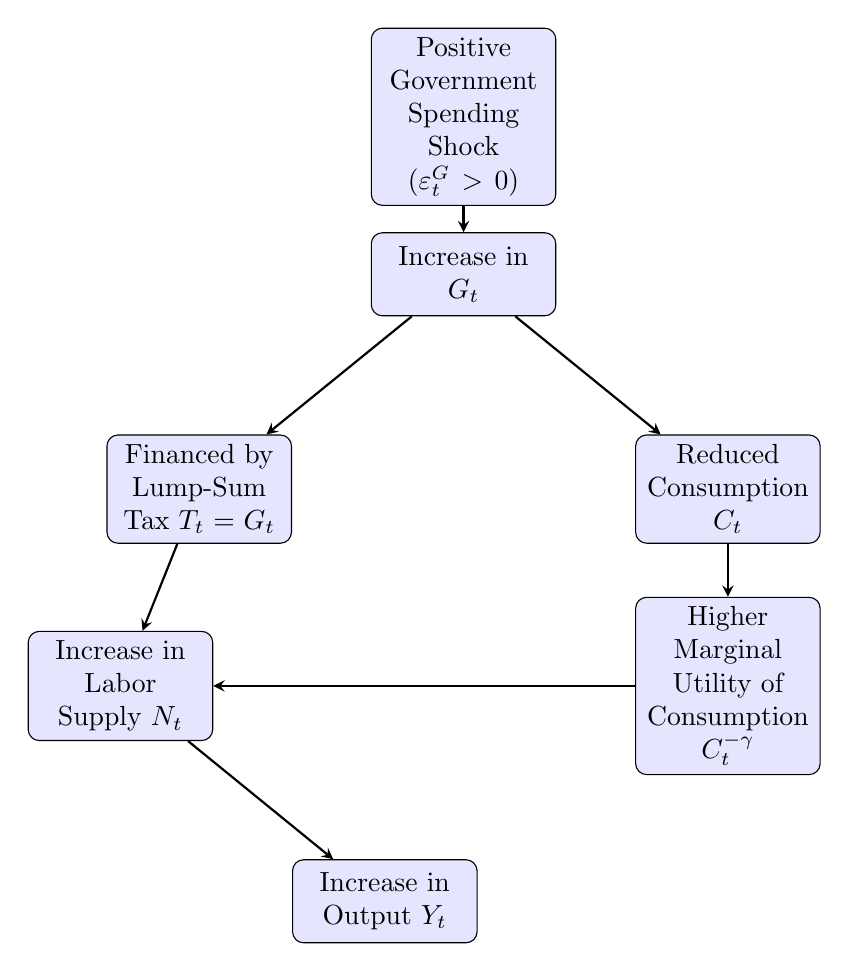
\begin{tikzpicture}[node distance = 2cm, auto]  
     % Nodes  
     \node [block] (shock) {Positive \\ Government Spending \\ Shock ($\varepsilon_t^G>0$)};  
     \node [block, below of=shock] (G) {Increase in \\ $G_t$};  
     \node [block, below left=1.5cm and 1cm of G] (tax) {Financed by \\ Lump-Sum Tax $T_t=G_t$};  
     \node [block, below right=1.5cm and 1cm of G] (cons) {Reduced \\ Consumption $C_t$};  
     \node [block, below of=cons, yshift=-0.5cm] (util) {Higher Marginal \\ Utility of Consumption \\ $C_t^{-\gamma}$};  
     \node [block, below of=tax, xshift=-1cm, yshift=-0.5cm] (lab) {Increase in \\ Labor Supply $N_t$};  
     \node [block, below right=1.5cm and 1cm of lab] (output) {Increase in \\ Output $Y_t$};  
       
     % Arrows  
     \draw [arrow] (shock) -- (G);  
     \draw [arrow] (G) -- (tax);  
     \draw [arrow] (G) -- (cons);  
     \draw [arrow] (cons) -- (util);  
     \draw [arrow] (util) -- (lab);  
     \draw [arrow] (tax) -- (lab);  
     \draw [arrow] (lab) -- (output);  
    \end{tikzpicture} 
    \caption{Transmission mechanism of a positive government spending shock (no capital case)}  
\end{figure}  
 
\begin{itemize}
    \item Capital case ($\alpha \neq 0$) : same dynamics as in the no capital case but the impact on output is stronger. We indeed have both a short term effect (adjust level of labor provided) and a long term effect (adjust capital stock lent to firms) to compensate for drop in disposable income for consumption.     
\end{itemize}

\subsection{NK model}

\subsection{Optimal monetary policy}
\subsubsection{Inefficient flex price allocation case : time varying $\theta_t$}
\begin{itemize}
    \item modification : $\theta$ is time-dependent so market power of firms can change from one period to the other and influence how high some firms will be able to price their goods. As the markup is updated at each period, it is impossible to compensate this inefficiency with a targeted subsidy. 
    \item modified log-linearized system : 
    \begin{enumerate}
        \item static price (flexible) : $p_t^{\diamond} = \mu_t^n+w_t-a_t$ with $\mu_t^n=ln(\frac{\theta_t(\theta-1)}{\theta(\theta_t-1)})$
        \item labor supply : $w_t-p_t-\gamma c_t=\psi n_t$ 
        \item labor demand (under flexible prices) : $n_t = c_t-a_t$ (does not depend on the firm!)
    \end{enumerate}
    \item flexible consumption $c_t^f$ is obtained from subsituting $n_t$ and $p_t$ in the labor supply equation
    \begin{equation}
        c_t^f= \frac{\psi +1}{\psi+\gamma}a_t - \frac{1}{\psi+\gamma}\mu_t^n
    \end{equation}
    \item dynamics : when $\theta_t$ goes down, the markup $\mu_t^n$ goes up and $c_t^f$ goes down 
    \item modified NKPC : 
    \begin{enumerate}
        \item start from this : 
    \begin{equation}
        \pi_t = \frac{(1-\lambda)(1-\lambda\beta)}{\lambda}(p_t^{\diamond}-p_t) + \beta E_t[\pi_{t+1}]
    \end{equation}
        \item replace $p_t^{\diamond}$ by its expression then replace $p_t$ using the labor supply equation
        \item replace $n_t$ using the labor demand equation and pull together terms to recover $c_t^f$
    \end{enumerate}
    \begin{expectedresultsbox}
        \textcolor{blue}{\textbf{expected result : }}$\pi_t = \frac{(1-\lambda)(1-\lambda\beta)}{\lambda}(\psi+\gamma)(c_t-c_t^f) + \beta E_t[\pi_{t+1}]$
    \end{expectedresultsbox}
    \item we find the Philipps curve remains unchanged ! 
\end{itemize}
\begin{shortbox}
    \begin{enumerate}
        \item flexible price allocation is inefficient ($c_t^f \neq c_t^e$)
        \item the static profit maximizing price changes and so does the equilibrium consumption under flexible prices
        \item the NKPC remains unchanged ! 
    \end{enumerate}
\end{shortbox}



\section{Math Appendix}
\subsection{Usual Taylor Expansions}
\begin{tabular}{c|c|c}
\toprule
Function $f(x)$ & Taylor Expansion form & ...with sums \\ 
\midrule 
$e^x$ & $1 + x + x^2 + \cdots$ & $\sum_{n=0}^\infty\frac{x^n}{n!}$ \\ 
\midrule
$\frac{1}{1-x}$ & $1 - x + x^2 - x^3 + \cdots$ & $\sum_{n=0}^\infty (-1)^nx^n$ \\ 
\midrule
$\frac{1}{1-x}$ & $1 + x + x^2 + x^3 + \cdots$ & $\sum_{n=0}^\infty x^n$ \\ 
\midrule
$\ln(1+x)$ & $x - \frac{x^2}{2} + \frac{x^3}{3} + \cdots$ & $\sum_{n=1}^\infty(-1)^{n-1}\frac{x^n}{n}$ \\ 
\bottomrule
\end{tabular}
\subsection{Geometric Series}
Geometric series take either of these 3 forms and give the following results (all can be admitted): 
\begin{equation}
\begin{aligned}
    1)& \sum_{k=0}^\infty q^k = \sum_{k=t}^\infty q^{k-t} = \frac{1}{1-q} \\
    2)& \sum_{k=0}^\infty kq^{k-1} = \frac{1}{(1-q)^2} \\
    3)& \sum_{k=0}^\infty k(k-1)q^{k-1} = \frac{2}{(1-q)^3}
\end{aligned}
\end{equation}
\subsection{Expectation indices and period notations}
\textbf{The t+i notation :} begins at time t\\

 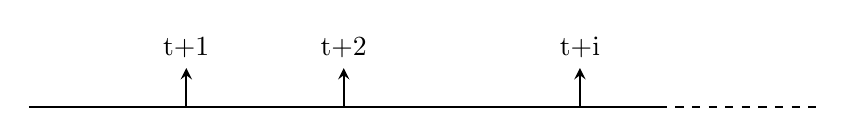
\begin{tikzpicture}[>=stealth, thick]  
   
   % Draw solid part of the timeline  
   \draw (0,0) -- (8,0);  
     
   % Draw dashed portion to indicate continuation  
   \draw[dashed] (8,0) -- (10,0);  
     
   % Add pointers at specific positions  
   \draw[->] (2,0) -- (2,0.5);  
   \draw[->] (4,0) -- (4,0.5);  
   \draw[->] (7,0) -- (7,0.5);  
   
   % Optionally, add time labels above the pointers if needed  
   \node[above] at (2,0.5) {t+1};  
   \node[above] at (4,0.5) {t+2};  
   \node[above] at (7,0.5) {t+i};  
   
 \end{tikzpicture}  \\
\underline{form of the sum :}
\begin{equation}
    E_t[\sum_{i=0}^\infty\beta^{i}X_{t+i}]
\end{equation}
\noindent\rule{\textwidth}{0.4pt}
 {\small  
 \textbf{Note :} {\scriptsize (1)
$\beta$ is indexed by i and not t+i because between period t and t+i, only i periods have passed so we discount i times. }\par\vspace{0.5cm}\par 
\noindent\textbf{The t notation :} begins at time 0\\

 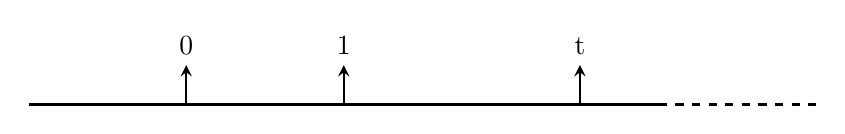
\begin{tikzpicture}[>=stealth, thick]  
   
   % Draw solid part of the timeline  
   \draw (0,0) -- (8,0);  
     
   % Draw dashed portion to indicate continuation  
   \draw[dashed] (8,0) -- (10,0);  
     
   % Add pointers at specific positions  
   \draw[->] (2,0) -- (2,0.5);  
   \draw[->] (4,0) -- (4,0.5);  
   \draw[->] (7,0) -- (7,0.5);  
   
   % Optionally, add time labels above the pointers if needed  
   \node[above] at (2,0.5) {0};  
   \node[above] at (4,0.5) {1};  
   \node[above] at (7,0.5) {t};  
   
 \end{tikzpicture} \\ 
\underline{form of the sum :}
\begin{equation}
    E_0[\sum_{t=0}^\infty\beta^{t}X_t]
\end{equation}
\textbf{The t, i notation :} begins at time t as well but each period is noted i instead of t+i\\
 \begin{tikzpicture}[>=stealth, thick]  
   
   % Draw solid part of the timeline  
   \draw (0,0) -- (8,0);  
     
   % Draw dashed portion to indicate continuation  
   \draw[dashed] (8,0) -- (10,0);  
     
   % Add pointers at specific positions  
   \draw[->] (2,0) -- (2,0.5);  
   \draw[->] (4,0) -- (4,0.5);  
   \draw[->] (7,0) -- (7,0.5);  
   
   % Optionally, add time labels above the pointers if needed  
   \node[above] at (2,0.5) {t};  
   \node[above] at (4,0.5) {t+1};  
   \node[above] at (7,0.5) {i};  
   
 \end{tikzpicture}  \\
\underline{form of the sum :}
\begin{equation}
    E_t[\sum_{i=t}^\infty\beta^{i-t}X_i]
\end{equation}

\end{document}

